% Typeset the method name over the original label positions; preserve all plot data.
\resizebox{!}{0.80\textheight}{%
\begin{tikzpicture}
  \node[anchor=south west,inner sep=0] (chart) at (0,0)
    {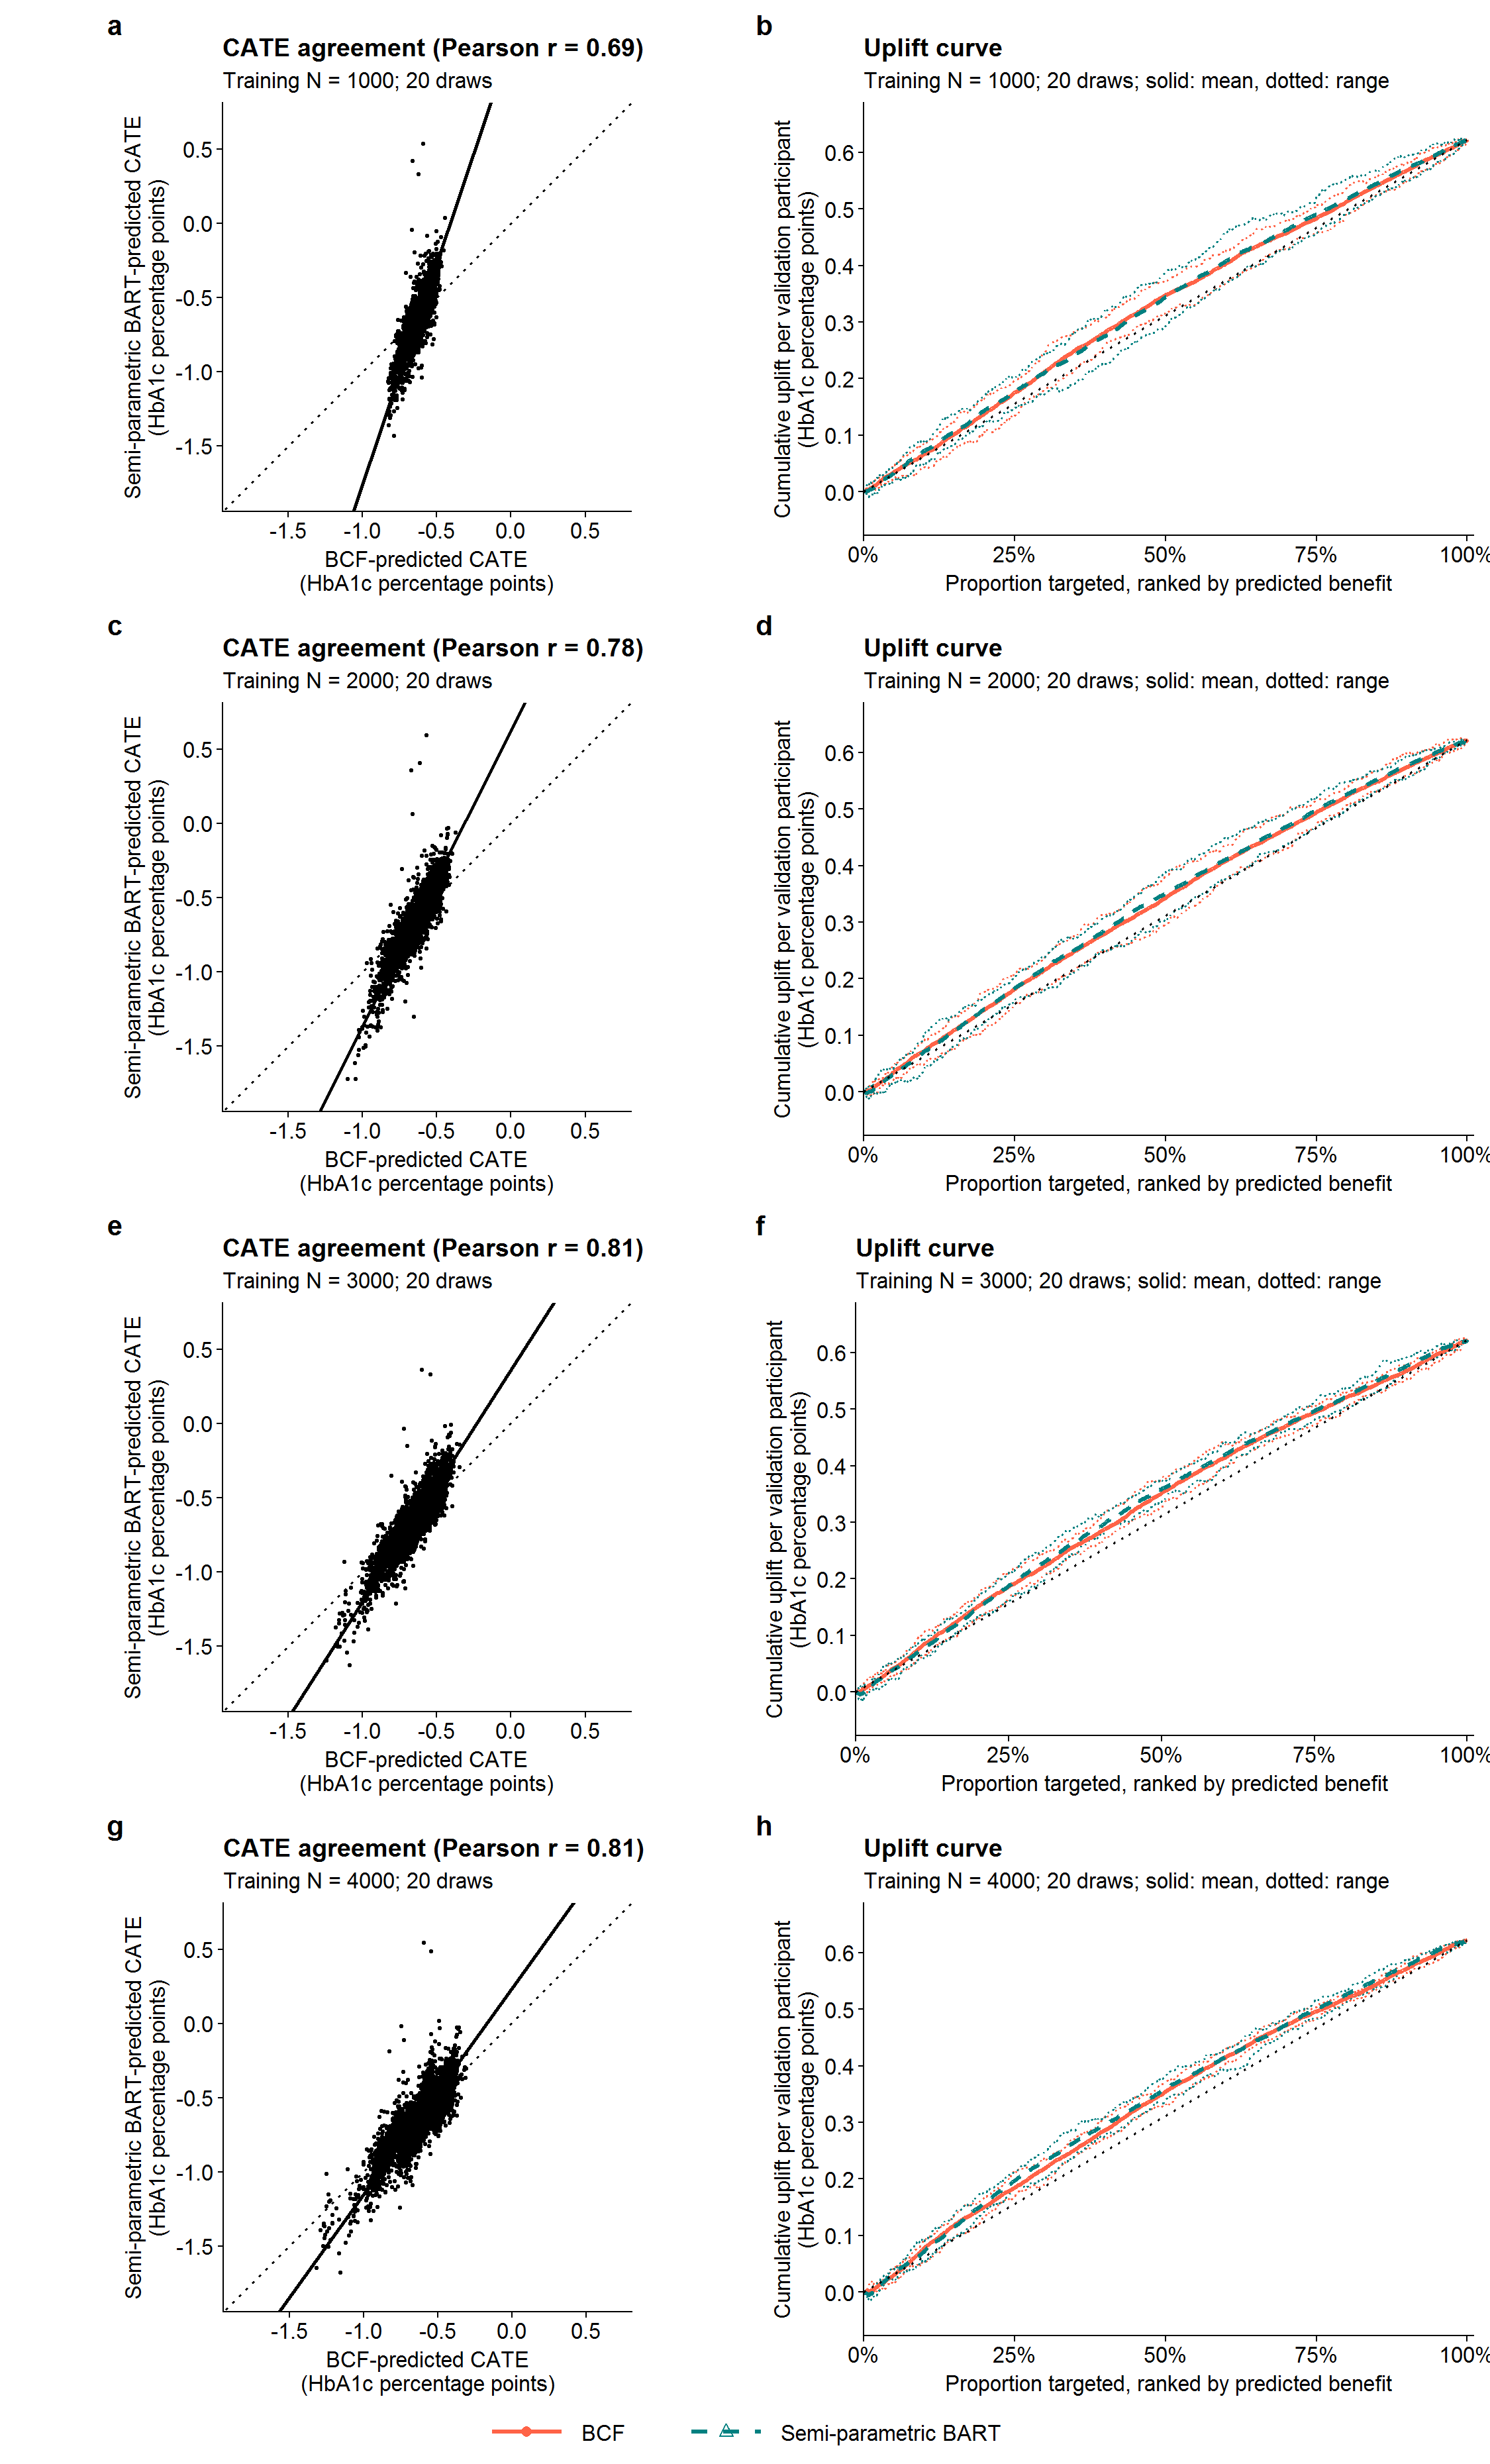
\includegraphics[width=7.5in]{canvas_hchs_gibbs_20260921_OOS_compound_N1000-2000-3000-4000.png}};
  \begin{scope}[x={(chart.south east)},y={(chart.north west)}]
    \foreach \top in {0,906,1812,2718} {
      \fill[white] (0.08178,{1-(755+\top)/3720}) rectangle
                   (0.09823,{1-(172+\top)/3720});
      \node[rotate=90,inner sep=0,font=\fontfamily{phv}\fontsize{8}{9.6}\selectfont]
        at (0.09,{1-(463.5+\top)/3720}) {B-SLIM-predicted CATE};
    }
    \fill[white] (0.52222,{1-3698/3720}) rectangle (0.67378,{1-3655/3720});
    \node[anchor=west,inner sep=0,font=\fontfamily{phv}\fontsize{8}{9.6}\selectfont]
      at (0.52444,{1-3676/3720}) {B-SLIM};
  \end{scope}
\end{tikzpicture}%
}
